\usetikzlibrary{arrows.meta}
\begin{frame}{ECN}
\begin{itemize}
\item explicit congestion notification
\vspace{.5cm}
\item when buffer `close' to full
\item switches set `congestion experienced' (CE) signal in some packets
\item goal: congestion signal \textit{instead of} packet drops
    \begin{itemize}
    \item avoid all the retransmission, hopefully
    \end{itemize}
\vspace{.5cm}
\item still have fallback to dropping packets
\end{itemize}
\end{frame}

\begin{frame}{ECN and TCP/IP}
\begin{itemize}
\item congestion experience (CE) signal in IP heaer
\item when ACKing, ``return'' CE signal with ACK
    \begin{itemize}
    \item ECN echo (ECE) TCP flag on ACK packets
    \end{itemize}
\vspace{.25cm}
\item when sender sees ECE flag, confirm reciept by setting
    ``congestion window reduced'' (CWR) flag until ECE flag stops being set
\end{itemize}
\end{frame}

\begin{frame}{ECN opt-in}
    \begin{itemize}
    \item two bits in IP header
    \item RFC 3168 says:
    \vspace{.5cm}
    \item \texttt{00} = not-ECN capable (default)
    \item \texttt{01}, \texttt{10} = ECN-capable (set by TCP/etc. implementation)
    \item \texttt{11} = congestion experienced
    \end{itemize}
\end{frame}

\begin{frame}{ECN timeline}
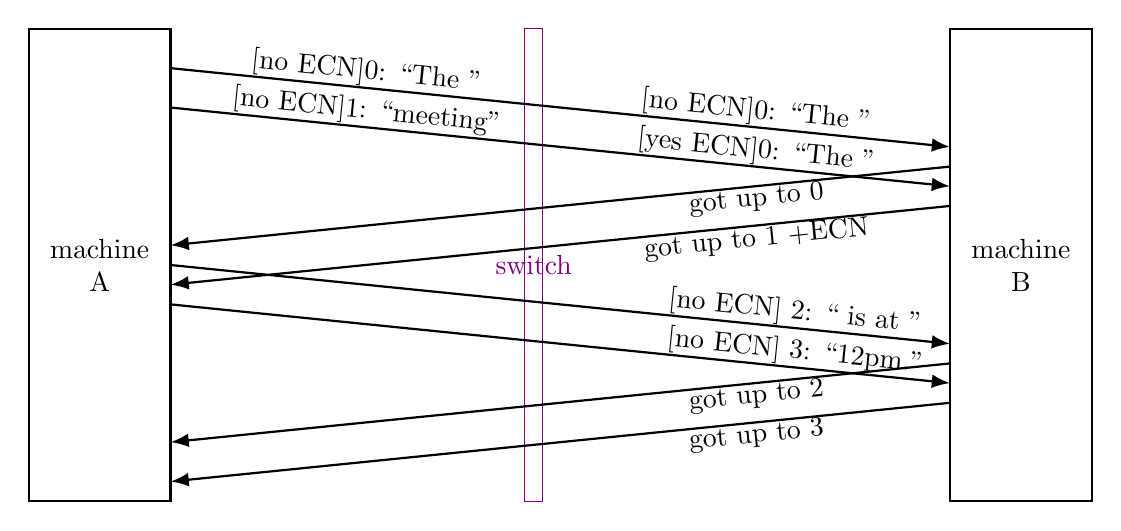
\begin{tikzpicture}
\tikzset{
    box/.style={thick},
    message/.style={draw,thick,-Latex},
    failure/.style={draw,ultra thick,red,cross out,minimum width=1cm,minimum height=1cm},
    every node/.style={inner sep=0.1mm},
}
\begin{scope}[xshift=1cm,x=0.9cm]
\draw[box] (0, 0) rectangle ++(2, -6) 
    node[midway,align=center] {machine\\A};
\draw[violet] (7, 0) rectangle ++(.25, -6) 
    node[midway,align=center] {switch};
\draw[box] (13, 0) rectangle ++(2, -6) 
    node[midway,align=center] {machine\\B};
\draw[message] (2, -0.5) -- (13, -1.5) node[pos=0.25,above,sloped] {[no ECN]{0}: ``The ''}
    node[pos=0.75,above,sloped] {[no ECN]{0}: ``The ''};
\draw[message] (13, -1.75) -- (2, -2.75) node[pos=0.25,sloped,below] {got up to {0}};
\draw[message] (2, -1) -- (13, -2) node[pos=0.25, above, sloped] {[no ECN]{1}: ``meeting''}
    node[pos=0.75,above,sloped] {\myemph{[yes ECN]}{0}: ``The ''};
\draw[message] (13, -2.25) -- (2, -3.25) node[pos=0.25, sloped,below] {got up to {1} \myemph{+ECN}};

% in response to got 0
\draw[message] (2, -3) -- (13, -4) node[pos=0.8, above, sloped] {[no ECN] {2}: `` is at ''};
\draw[message] (13, -4.25) -- (2, -5.25) node[pos=0.25, sloped,below] {got up to {2}};
% in response to got 1
\draw[message] (2, -3.5) -- (13, -4.5) node[pos=0.8, above, sloped] {[no ECN] {3}: ``12pm.''};
\draw[message] (13, -4.75) -- (2, -5.75) node[pos=0.25, sloped,below] {got up to {3}};
\end{scope}
\end{tikzpicture}
\begin{itemize}
\item data sent has place for ECN bit to be placed
\item switch modifies ECN bit \myemph{if buffer close to full}
\item ACK indicates if ECN bit was set
\end{itemize}
\end{frame}

\begin{frame}{reacting to ECN marks}
    \begin{itemize}
    \item multiple options for using ECN marks
    \item simplest idea:
    \vspace{.5cm}
    \item adjust window as if packet was dropped
    \item \ldots but don't need to resend data
    \end{itemize}
\end{frame}

\begin{frame}{ECN deployment}
    \begin{itemize}
    \item ECN proposed in 2001
    \item 13 years later: around 56\% support on websites\footnote{Trammel et al, ``Enabling Internet-Wide Deployment of Explicit Congestion Notification''}
    \item 16 years later: 
        \begin{itemize}
        \item around 80\% support on websites\footnote{K\"uhlewind et al, ``Tracing Internet Path Transparency''}
        \item around 0.2\% of servers disallow connection when ECN requested
        \end{itemize}
    \item 20 years later:
        \begin{itemize}
        \item around 86\% support on websites\footnote{Lim et al, ``A Fresh Look at ECN Traversal in the Wild''}
        \item around 4\% of paths strip ECN signals, including notable ISPs/cloud providers/etc.
        \item around 7.5\% of connections (from sampled Universities) enable ECN
        \end{itemize}
    \end{itemize}
\end{frame}

% FIXME: ECN-capable mark

\begin{frame}{example: DCTCP}
    \begin{itemize}
    \item DataCenter TCP (2010)
    \item intended for datacenters
        \begin{itemize}
        \item high bandwidth, low latency networks
        \end{itemize}
    \item based on explicit congestion notification
    \item \ldots but uses different multiplicative decrease strategy
    \vspace{.5cm}
    \item measure portion of packets marked recently $\alpha$ 
    \item decrease by factor of $1-\alpha/2$
        \begin{itemize}
        \item respond gradually to congestion
        \item start responding early (packets marked when queues far from full)
        \end{itemize}
    \end{itemize}
\end{frame}
